\section{Gaits}
\subsection*{Inplace hopping}
\begin{frame}
\frametitle{In-place hopping}
\begin{block}{Controller}
\begin{itemize}
  \item 
  Impact torque destabilizing, control robot attitude\\[0.1in]
  \item
  Flight, spring phases : $\theta_d = 0$\\[0.1in]
  \item
  Stance phase,
  \begin{equation*}
   \theta_d = \tan^{-1}\left(\frac{x_{impact}}{h_{max}}\right)
  \end{equation*}\\[0.1in]
\end{itemize}
  
  \begin{columns}
  \column{0.5\textwidth} 
  \begin{figure}
  \centering
  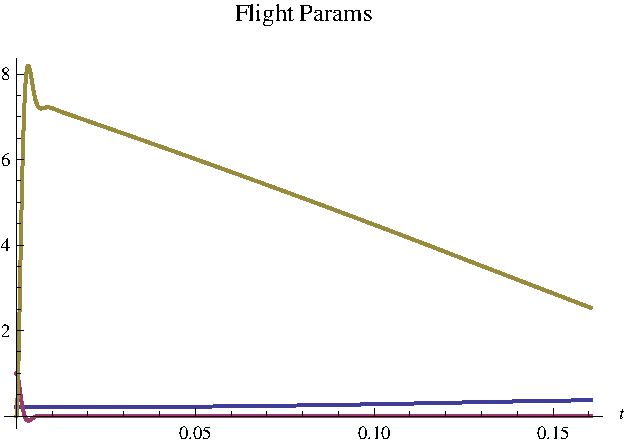
\includegraphics[scale=0.45]{fig/inplace_pFlight_params.pdf}
  \end{figure}
  
  \column{0.5\textwidth} 
  \begin{figure}
  \centering
  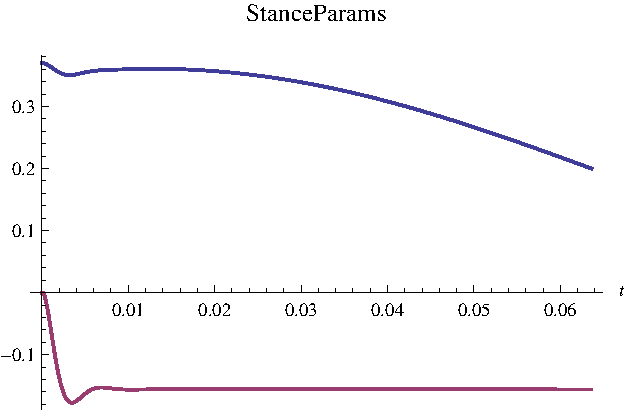
\includegraphics[scale=0.45]{fig/inplace_pStance_params.pdf}
  \end{figure}
  \end{columns}
  \begin{itemize}
    {
    \small
    \item 
    $l(t)$ - Blue, $\theta(t)$ - Pink, $\phi(t)$ - Yellow, t = secs
    }
  \end{itemize}

\end{block}

\end{frame}

\begin{frame}
\frametitle{Inplace : Trajectory}
\begin{itemize}
 \item
  Start at $y = 1$m, $\theta = 1$ rad, $\dot{\theta} = -1$ rad/s
\end{itemize}
  \begin{figure}
  \centering
  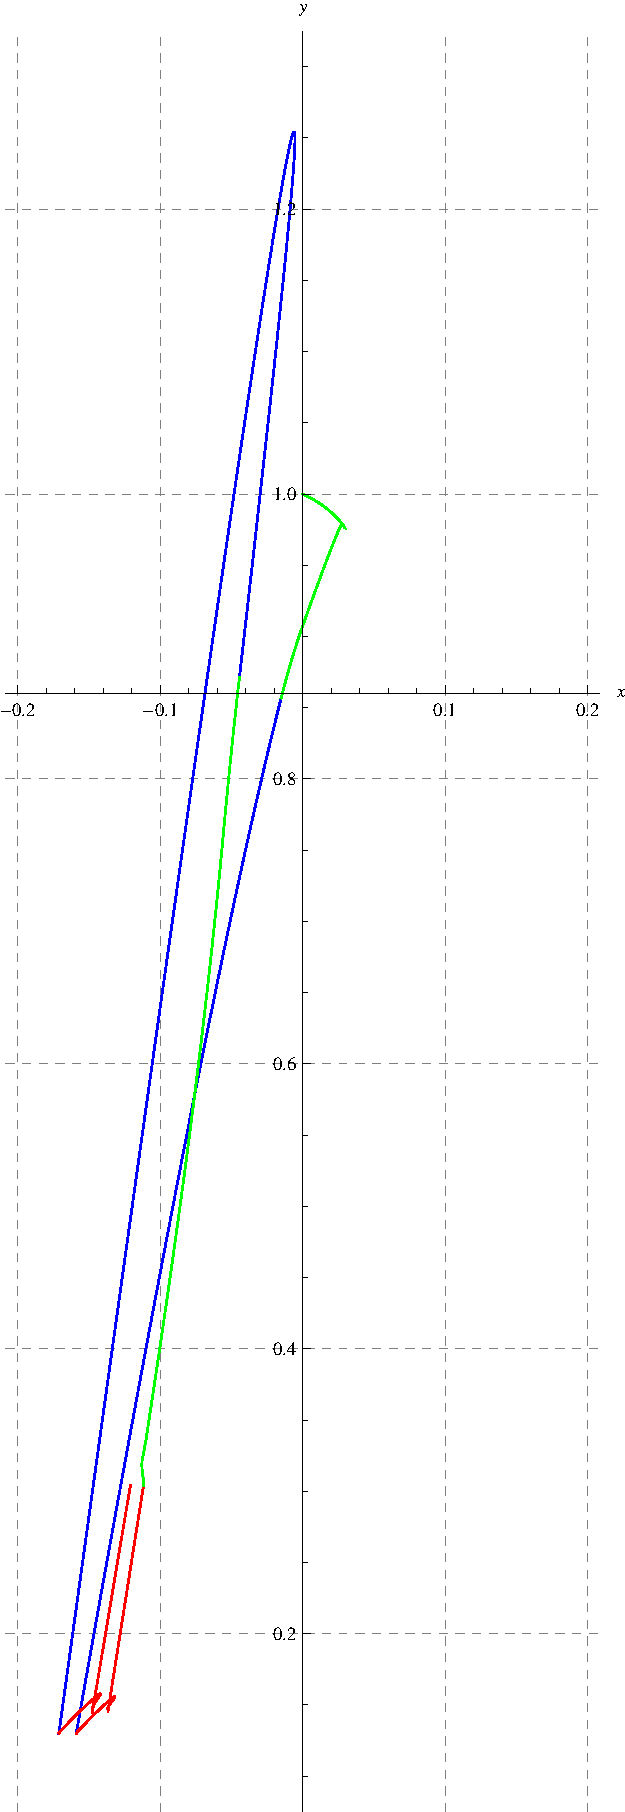
\includegraphics[scale=0.2]{fig/plot_inplace.pdf}
  \caption{Inplace : Trajectory}
  \end{figure} 
\end{frame}

\subsection*{Running}
\begin{frame}
\frametitle{Stance controller}
\begin{block}{Details}
\begin{itemize}
  \item
  Most important phase for control\\[0.1in]
  \item
  Generate $\theta_G(t)$ using good initial conditions\\[0.1in]
  \item
  PID torque controller for $e = \theta - \theta_G$\\[0.1in]
\end{itemize}
  \begin{figure}
  \centering
  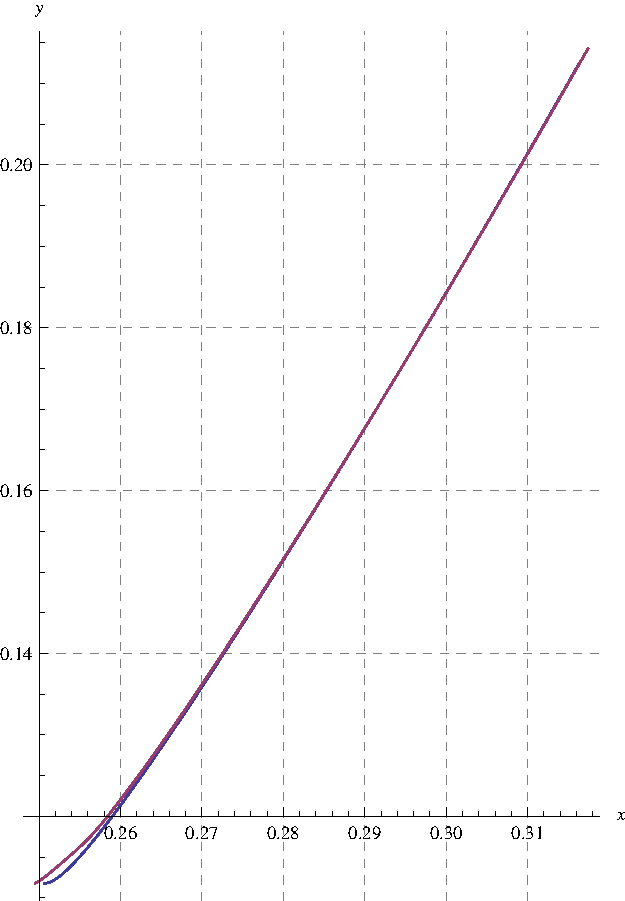
\includegraphics[scale=0.4, angle = 270]{fig/pStance_trajec_control.pdf}
  \caption{Good - Blue, Perturbed - Pink, distances in meters}
  \label{fig:stance_control_trajec}
  \end{figure}

\end{block}
\end{frame}

\begin{frame}
\frametitle{Flight, Spring phases}
\begin{block}{Control}
\begin{itemize}
  \item
  Large time--scales\\[0.1in]
  \item
  Solve attitude reorientation to impact attitude\\[0.1in]
\end{itemize}
  \begin{equation*}
     \Delta\;\theta (t)= \theta_{impact} - \theta(t)
    \end{equation*}\\[0.1in]
    \begin{equation*}
    \ddot{\phi}_d(t) = \left(\frac{-2\;J_b}{J_w}\right) \left(\frac{\Delta\;\theta - \dot{\theta}(t)\;t_{left}}{t_{left}^2}\right)
    \end{equation*}\\[0.1in]

    \begin{equation*}
     e(t) = \ddot{\phi}(t) - \ddot{\phi}_d(t)
    \end{equation*}
    \begin{equation*}
     U_{\phi}(t) = \ddot{\phi}_d(t) + K_p\;e(t) + K_d\;\dddot{\phi}(t) + K_i\;\;\int \phi dt
    \end{equation*}
\end{block}
\end{frame}

\begin{frame}
  \frametitle{Controlled trajectory}
  \begin{itemize}
    \item
    Perturb attitude at liftoff
  \end{itemize}

  \begin{figure}
  \centering
  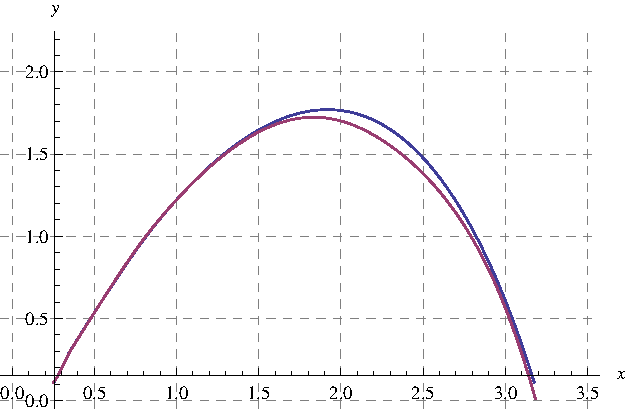
\includegraphics[scale=0.8]{fig/pFullTrajec_control.pdf}
  \caption{Trajectory Controller : Good - Blue, Perturbed - Pink}
  \label{fig:full_trajec_control}
  \end{figure}

\end{frame}
